\documentclass[11pt,letterpaper]{article}

\usepackage[T1]{fontenc}
\usepackage[utf8]{inputenc}
\usepackage{newtxtext,newtxmath}
\usepackage[margin=1in]{geometry}
\usepackage{microtype}
\usepackage{amsmath}
\usepackage{booktabs,tabularx,longtable,array}
\usepackage[table]{xcolor}
\usepackage{enumitem}
\usepackage{caption}
\usepackage{xspace}
\usepackage{tikz}
\usetikzlibrary{arrows.meta,positioning}
\usepackage[numbers,sort&compress]{natbib}
\usepackage[hidelinks]{hyperref}
\usepackage[nameinlink,capitalise]{cleveref}

% QRED's venue is indexed under its Chinese title; print the journal's English name instead
\DeclareUnicodeCharacter{7DB2}{}\DeclareUnicodeCharacter{969B}{Journal of Internet Technology}
\DeclareUnicodeCharacter{8DEF}{}\DeclareUnicodeCharacter{6280}{}\DeclareUnicodeCharacter{8853}{}
\DeclareUnicodeCharacter{5B78}{}\DeclareUnicodeCharacter{520A}{}

\definecolor{accent}{HTML}{1D4ED8}
\definecolor{muted}{HTML}{525252}
\hypersetup{colorlinks=true,linkcolor=accent,citecolor=accent,urlcolor=accent}
\setlist{itemsep=2pt,topsep=4pt}
\captionsetup{font=small,labelfont=bf}
\newcolumntype{L}[1]{>{\raggedright\arraybackslash}p{#1}}
\newcolumntype{Y}{>{\raggedright\arraybackslash}X}
\newcommand{\RQ}[1]{\textbf{RQ#1}}

% numbers generated by review/scripts/select_top50.py (do not edit by hand)
% generated by review/scripts/select_top50.py (do not edit by hand)
\newcommand{\nAllIdentified}{2{,}459\xspace}
\newcommand{\nAllIdentifiedDB}{567\xspace}
\newcommand{\nAllIdentifiedOther}{1{,}892\xspace}
\newcommand{\nAllReports}{396\xspace}
\newcommand{\nFlowAfterDup}{2{,}396\xspace}
\newcommand{\nFlowAssessed}{427\xspace}
\newcommand{\nFlowBackward}{151\xspace}
\newcommand{\nFlowDup}{63\xspace}
\newcommand{\nFlowExFT}{31\xspace}
\newcommand{\nFlowExTA}{1{,}954\xspace}
\newcommand{\nFlowForward}{275\xspace}
\newcommand{\nFlowForwardFound}{446\xspace}
\newcommand{\nFlowKnown}{6\xspace}
\newcommand{\nFlowNotRet}{15\xspace}
\newcommand{\nFlowSought}{442\xspace}
\newcommand{\nFlowUpdate}{1{,}460\xspace}
\newcommand{\nRestAB}{249\xspace}
\newcommand{\nRestCode}{18\xspace}
\newcommand{\nRestDesign}{282\xspace}
\newcommand{\nRestEmp}{310\xspace}
\newcommand{\nRestEmu}{34\xspace}
\newcommand{\nRestFT}{62\xspace}
\newcommand{\nRestFair}{51\xspace}
\newcommand{\nRestFormal}{2\xspace}
\newcommand{\nRestGen}{28\xspace}
\newcommand{\nRestHybrid}{78\xspace}
\newcommand{\nRestKN}{1\xspace}
\newcommand{\nRestKnown}{204\xspace}
\newcommand{\nRestMedian}{1\xspace}
\newcommand{\nRestN}{312\xspace}
\newcommand{\nRestNR}{106\xspace}
\newcommand{\nRestPctCode}{6\xspace}
\newcommand{\nRestPctFT}{20\xspace}
\newcommand{\nRestPctFair}{18\xspace}
\newcommand{\nRestPctGen}{10\xspace}
\newcommand{\nRestPctHybrid}{28\xspace}
\newcommand{\nRestPctRealKnown}{19\xspace}
\newcommand{\nRestPctSimKnown}{64\xspace}
\newcommand{\nRestPctSince}{70\xspace}
\newcommand{\nRestReal}{39\xspace}
\newcommand{\nRestSim}{131\xspace}
\newcommand{\nRestSince}{218\xspace}
\newcommand{\nTopAB}{29\xspace}
\newcommand{\nTopActBitrate}{6\xspace}
\newcommand{\nTopActCwnd}{13\xspace}
\newcommand{\nTopActNet}{4\xspace}
\newcommand{\nTopActParam}{8\xspace}
\newcommand{\nTopActRate}{12\xspace}
\newcommand{\nTopCiteMedian}{52.5\xspace}
\newcommand{\nTopCode}{7\xspace}
\newcommand{\nTopContribAnalysis}{3\xspace}
\newcommand{\nTopContribFramework}{4\xspace}
\newcommand{\nTopCtrlSender}{33\xspace}
\newcommand{\nTopCut}{27\xspace}
\newcommand{\nTopDeploy}{5\xspace}
\newcommand{\nTopDesign}{43\xspace}
\newcommand{\nTopEmp}{48\xspace}
\newcommand{\nTopEmu}{11\xspace}
\newcommand{\nTopFT}{19\xspace}
\newcommand{\nTopFair}{12\xspace}
\newcommand{\nTopFormal}{2\xspace}
\newcommand{\nTopFour}{6\xspace}
\newcommand{\nTopGDataCenter}{3\xspace}
\newcommand{\nTopGInternetGeneric}{36\xspace}
\newcommand{\nTopGIotAdHocSensor}{4\xspace}
\newcommand{\nTopGSatelliteSpace}{1\xspace}
\newcommand{\nTopGWirelessCellular}{6\xspace}
\newcommand{\nTopGen}{7\xspace}
\newcommand{\nTopHybrid}{15\xspace}
\newcommand{\nTopKN}{2\xspace}
\newcommand{\nTopKnown}{42\xspace}
\newcommand{\nTopMax}{497\xspace}
\newcommand{\nTopMedian}{2\xspace}
\newcommand{\nTopN}{50\xspace}
\newcommand{\nTopNR}{6\xspace}
\newcommand{\nTopNoCount}{9\xspace}
\newcommand{\nTopPctCode}{16\xspace}
\newcommand{\nTopPctFT}{38\xspace}
\newcommand{\nTopPctFair}{28\xspace}
\newcommand{\nTopPctGen}{16\xspace}
\newcommand{\nTopPctHybrid}{35\xspace}
\newcommand{\nTopPctRealKnown}{43\xspace}
\newcommand{\nTopPctSimKnown}{31\xspace}
\newcommand{\nTopPctSince}{8\xspace}
\newcommand{\nTopReal}{18\xspace}
\newcommand{\nTopRest}{312\xspace}
\newcommand{\nTopRestOfSettings}{14\xspace}
\newcommand{\nTopSim}{13\xspace}
\newcommand{\nTopSince}{4\xspace}
\newcommand{\nTopStudies}{362\xspace}
\newcommand{\nTopTied}{4\xspace}

\xspaceaddexceptions{\%}

\title{\textbf{Reinforcement Learning for Congestion Control}\\[4pt]
\Large A Review of the \nTopN Most-Cited Studies}
\author{Gaurab Baral \and Nityashree Vangala}
\date{CS 6043: Networking\\[2pt] Fall 2026}

\begin{document}
\maketitle

\begin{abstract}
Reinforcement learning (RL) lets a congestion controller learn its control law from experience. Our searches identified \nAllIdentified records and \nTopStudies primary studies of RL and imitation learning for congestion control published from 2016 to 2026. Because of time constraints, this report reviews the \nTopN of those studies with the most citations in a single Semantic Scholar snapshot taken on 9~November~2026. We ask how these controllers are designed, how they are tested, and what keeps operators from using them. Of the \nTopDesign design studies, \nTopCtrlSender run at the sender and \nTopHybrid keep a classic algorithm or safeguard in the deployed control loop. Of the \nTopKnown studies whose evaluation level we could determine, \nTopReal (\nTopPctRealKnown\%) reach a real network. Only \nTopGen design studies test outside their training distribution and only \nTopCode release code. Five report production use or tests with real users. Four of those keep a classic component in the loop, and the fifth learned from logged sessions. Citation ranking favors older work: only \nTopSince of the \nTopN studies first appeared in 2023 or later, against \nRestPctSince\% of the remaining studies. Our findings therefore describe the literature's most influential papers and should not be read as a census of current practice.
\end{abstract}

% ======================================================================
\section{Introduction}
\label{sec:intro}

\subsection{Motivation}
\label{sec:motivation}

Congestion control (CC) decides how fast a sender may send its data into a shared network. It is one of the oldest control problems in networking. After major Internet congestion in 1986, Jacobson's slow start and additive-increase/multiplicative-decrease (AIMD) methods helped stabilize the network by adjusting sending rates when packets were lost~\cite{jacobson1988congestion,chiu1989analysis}. Almost four decades later the problem takes many forms. Today, data travels over gigabit fiber, shared Wi-Fi, cellular networks whose capacity changes every few milliseconds, satellite networks that frequently switch connections between satellites~\cite{narayanan2020first,mohan2024multifaceted}, and data-center networks where a round trip takes only tens of microseconds. Despite these advances, congestion remains difficult to manage. Some challenges in CC include packet loss unrelated to congestion, noisy delay measurements, and widely varying buffer sizes~\cite{gettys2012bufferbloat,jiang2012tackling}. These challenges have led researchers to design algorithms for specific environments: Vegas, CUBIC, BBR and Copa for the Internet, Sprout, Verus and ABC for wireless networks, and DCTCP, DCQCN, TIMELY, HPCC, Swift, PowerTCP and Bolt for data centers~\cite{haile2021endtoend,zhou2026endtoend}.

With reinforcement learning (RL), a controller learns its control law instead of having it written by hand. In RL-based congestion control, an agent at the sender (or in the network) watches signals such as delay, throughput, and packet loss. Every short interval this agent raises or lowers the sending rate or the congestion window, and it receives a reward that is high for fast delivery and low for long delays or lost packets. Over many trials it learns which action works best in each network state. Remy~\cite{winstein2013remy} and PCC~\cite{dong2015pcc,dong2018vivace} showed that machine-generated or online-learned controllers can beat hand-tuned ones. Aurora~\cite{jay2019aurora} then cast Internet congestion control explicitly as a deep RL problem in 2018--2019, and the field has grown quickly since.

Our searches retrieved \nAllIdentified records, and \nTopStudies primary studies met our eligibility criteria (\cref{sec:method}). However, learned controllers that look excellent in a simulator sometimes fail on network links they never saw. Few of them run inside an operating-system kernel, and fewer still have been deployed by an operator. Due to time constraints, we examine only the \nTopN studies with the most citations.

\subsection{Research questions and contributions}
\label{sec:rqs}

We organize the survey around three research questions.

\begin{description}[leftmargin=1.2cm,labelwidth=1cm]
  \item[\RQ{1}] \textbf{Design.} How do RL methods control congestion: what do they observe, what do they change, and what reward do they learn from?
  \item[\RQ{2}] \textbf{Testing.} How are these methods trained and tested, and do they still work on networks they did not see in training?
  \item[\RQ{3}] \textbf{Deployment.} What stops operators from using RL-based congestion control in real networks, and what research could fix these problems?
\end{description}

\noindent This report contributes a reproducible ranking of the \nTopStudies eligible studies by citations, a design and evidence profile of the top \nTopN (\cref{sec:wan,sec:testing}, \cref{app:list}), a comparison of those \nTopN with the other \nTopRest (\cref{tab:compare}), and an analysis of the barriers to deployment that the \nTopN expose (\cref{sec:deployment}).

\subsection{Congestion control}
\label{sec:cc}

A congestion controller should use the available bottleneck capacity, avoid standing queues and loss, share capacity among competing flows, converge quickly when conditions change, and coexist with the deployed base, which in practice means not starving CUBIC and BBR flows. Fairness is often measured with Jain's index~\cite{jain1984fairness}. Ware et al.\ argue that deployability should instead be judged by the \emph{harm} a new algorithm does to existing traffic~\cite{ware2019beyond}.

End-to-end controllers infer congestion from what they can measure: packet loss, round-trip time (RTT) and its trend, delivery rate, and Explicit Congestion Notification (ECN) marks set by routers~\cite{rfc3168}. They act through the \emph{congestion window} (cwnd), which caps the data in flight, or the \emph{pacing rate}, which spaces packets in time.

Reno halves cwnd on loss and grows it by one packet per RTT~\cite{rfc5681}. CUBIC, the Linux default, grows cwnd as a cubic function of the time since the last loss~\cite{ha2008cubic}. Vegas and Copa back off when the RTT rises above its minimum~\cite{brakmo1995vegas,arun2018copa}. BBR estimates the bottleneck bandwidth and minimum RTT and paces at the estimated bandwidth~\cite{cardwell2016bbr}. Routers and switches take part through active queue management (AQM), which drops or marks packets before the buffer fills, as in RED, CoDel and PIE~\cite{floyd1993red,nichols2012codel,rfc8033}. In data centers, DCTCP reacts to the fraction of ECN-marked packets~\cite{alizadeh2010dctcp}, and its performance depends on a marking threshold that operators usually tune by hand.

\subsection{Reinforcement learning}
\label{sec:rl}

RL formalizes sequential decision making as a Markov decision process: at each step the agent observes a state $s_t$, takes an action $a_t$ from its policy $\pi$, receives a reward $r_t$, and the environment moves to $s_{t+1}$. The goal is a policy that maximizes the expected discounted return $\mathbb{E}[\sum_t \gamma^t r_t]$~\cite{sutton2018reinforcement}. A sender sees only its own feedback, so congestion control is formally partially observable~\cite{kaelbling1998planning}. Most designs compensate by feeding the agent a short history of observations. The \nTopN studies use the following families of methods.

\begin{itemize}
  \item \textbf{Value-based methods} learn the action-value function $Q(s,a)$. Tabular Q-learning suits small discrete state spaces, and the Deep Q-Network (DQN)~\cite{mnih2015human} approximates $Q$ with a neural network.
  \item \textbf{Policy-gradient methods} optimize $\pi$ directly. PPO~\cite{schulman2017ppo} and A3C~\cite{mnih2016a3c} handle continuous rate multipliers naturally.
  \item \textbf{Off-policy actor-critic methods} such as DDPG~\cite{lillicrap2016ddpg} and TD3~\cite{fujimoto2018td3} reuse past experience from a replay buffer. IMPALA~\cite{espeholt2018impala} decouples acting from learning.
  \item \textbf{Offline RL} learns from a fixed dataset of logged interactions without exploring online~\cite{levine2020offline}.
  \item \textbf{Imitation learning} trains a policy to copy an expert, which can be an oracle with full knowledge of a simulated link or an existing heuristic~\cite{ross2011dagger}.
  \item \textbf{Bandits} treat each decision interval as a single-step problem.
  \item \textbf{Multi-agent RL} trains several interacting agents, for example competing flows or switches~\cite{zhang2021multi}.
  \item \textbf{Multi-objective RL} learns one policy for many trade-offs~\cite{hayes2022practical}.
\end{itemize}

\subsection{Congestion control as an RL problem}
\label{sec:formulation}

\Cref{fig:loop} shows the formulation that Aurora made popular~\cite{jay2019aurora}. Time is divided into \emph{monitor intervals}. The agent picks an action at the start of each interval, and when the ACKs for that interval return, the sender computes statistics and the reward. Designs vary in five respects.

\begin{figure}[t]
\centering
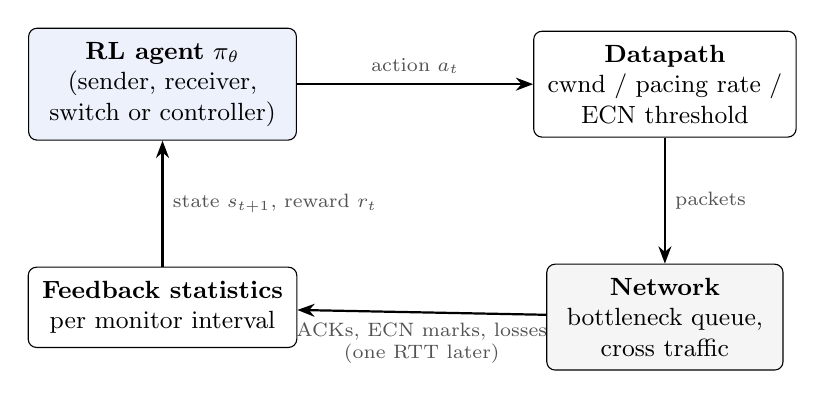
\begin{tikzpicture}[
  box/.style={draw, rounded corners=3pt, align=center, minimum height=10mm, inner sep=5pt, font=\small},
  lab/.style={font=\scriptsize, align=center, text=muted},
  >={Stealth[length=2.2mm]}]
  \node[box, fill=accent!8, minimum width=34mm] (agent) {\textbf{RL agent} $\pi_\theta$\\ (sender, receiver,\\ switch or controller)};
  \node[box, right=30mm of agent, minimum width=30mm] (dp) {\textbf{Datapath}\\ cwnd / pacing rate /\\ ECN threshold};
  \node[box, below=16mm of dp, minimum width=30mm, fill=black!4] (net) {\textbf{Network}\\ bottleneck queue,\\ cross traffic};
  \node[box, below=16mm of agent, minimum width=34mm] (stats) {\textbf{Feedback statistics}\\ per monitor interval};
  \draw[->, thick] (agent) -- node[above, lab]{action $a_t$} (dp);
  \draw[->, thick] (dp) -- node[right, lab]{packets} (net);
  \draw[->, thick] (net) -- node[below, lab]{ACKs, ECN marks, losses\\(one RTT later)} (stats);
  \draw[->, thick] (stats) -- node[right, lab]{state $s_{t+1}$, reward $r_t$} (agent);
\end{tikzpicture}
\caption{The usual RL congestion-control loop. The agent acts once per monitor interval and observes the consequences one RTT later.}
\label{fig:loop}
\end{figure}

\begin{enumerate}
  \item \textbf{Placement.} Most agents run at the sender. Some run at the receiver, which is common for real-time video. Others sit in switches and routers or in a central controller.
  \item \textbf{Observation.} Typical inputs are a short history of throughput, RTT, RTT gradient, loss rate and the current cwnd or rate. Aurora chose scale-free features (latency gradient, latency ratio and sending ratio) to help generalization across link speeds.
  \item \textbf{Action.} The action can set the cwnd or rate, tune a parameter of a classic algorithm, select among existing algorithms, or set a network parameter such as an ECN threshold.
  \item \textbf{Objective.} Most rewards combine throughput, delay and loss. Aurora uses $10\cdot\text{throughput} - 1000\cdot\text{latency} - 2000\cdot\text{loss}$. The reward fixes the operating point, so it acts as the controller's specification.
  \item \textbf{Decision frequency.} Neural inference on every ACK is too expensive at line rate, so most designs act once per interval.
\end{enumerate}

\noindent The consequences of an action arrive one RTT later and mix with the effects of other flows, so credit assignment is noisy. A controller also runs on networks whose statistics differ from any training environment, which makes performance under distribution shift a central measure of quality.

\subsection{Review method}
\label{sec:method}

The protocol query was
\begin{center}
\small\texttt{("reinforcement learning" OR "imitation learning") AND}\\
\small\texttt{("congestion control" OR "congestion window" OR "ECN")}
\end{center}
applied to titles and abstracts of works published 2016--2026. The database and citation searches were run on 31~October~2026, and an update search with broadened terms on 9~November~2026. Search strings in each source's syntax are given in \cref{app:search}.

We followed the PRISMA~2020 reporting guideline~\cite{page2021prisma}, with the search and snowballing steps adapted to computer science as recommended by Kitchenham and Charters~\cite{kitchenham2007guidelines} and Wohlin~\cite{wohlin2014snowballing}. The whole pipeline is in the replication code file that we submit with this survey.

\paragraph{Eligibility.} We included primary studies, in English, in which an RL or imitation-learning method (including bandits, offline RL and multi-agent RL) controls congestion in a packet network, along with studies that evaluate such controllers and frameworks built to train or test them. We excluded congestion outside packet networks, RL for other networking tasks such as routing or adaptive-bitrate video over TCP, methods with no RL component, and secondary studies.

\paragraph{Selection of the \nTopN.} \Cref{fig:flow} shows the flow. Reviewing the top \nTopN is a deviation from our protocol, which covered every eligible study. For each of the \nTopStudies studies we retrieved citation counts from the Semantic Scholar API on 9~November~2026, so that all counts come from one source on one date. Lookups used the DOI or arXiv identifier, or an exact title match when neither resolved. When a study has several linked reports, such as a conference paper and its journal extension, we used the highest count among them and did not add the counts, because such reports can share citing papers. Ties were broken by earlier publication year and then by study identifier. The cutoff is \nTopCut citations, and \nTopTied studies are tied at that value, so the tie-break decided two of the last places. Semantic Scholar had no record for \nTopNoCount studies. We checked them in OpenAlex, where none has more than seven citations, so none could have reached the cutoff.

\begin{figure}[t]
\centering
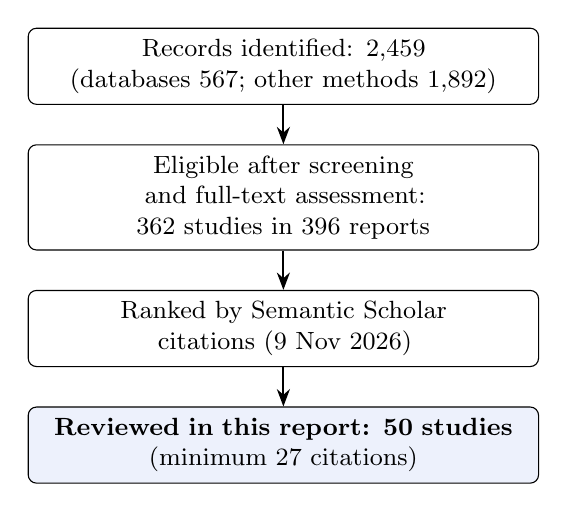
\begin{tikzpicture}[
  box/.style={draw, rounded corners=3pt, align=center, text width=62mm, minimum height=9mm, inner sep=4pt, font=\small},
  >={Stealth[length=2.2mm]}, node distance=5mm]
  \node[box] (a) {Records identified: \nAllIdentified\\ (databases \nAllIdentifiedDB; other methods \nAllIdentifiedOther)};
  \node[box, below=of a] (b) {Eligible after screening and full-text assessment:\\ \nTopStudies studies in \nAllReports reports};
  \node[box, below=of b] (c) {Ranked by Semantic Scholar citations (9 Nov 2026)};
  \node[box, below=of c, fill=accent!8] (d) {\textbf{Reviewed in this report: \nTopN studies}\\ (minimum \nTopCut citations)};
  \draw[->, thick] (a) -- (b); \draw[->, thick] (b) -- (c); \draw[->, thick] (c) -- (d);
\end{tikzpicture}
\caption{Selection of the studies reviewed in this report. The full PRISMA flow, with exclusion counts and reasons, is in the replication package.}
\label{fig:flow}
\end{figure}

\paragraph{Data items and appraisal.} For each study we coded the setting, control point, RL method, state, action, reward and training setup. We also coded the highest evaluation level reached: \emph{simulation} (a discrete-event or fluid model), \emph{emulation} (real protocol stacks over emulated links) or \emph{real network} (real links or production traffic). Finally, we coded whether generalization outside the training range was tested, whether fairness was evaluated, and whether code was released. We call a design \emph{hybrid} when a classic algorithm or safeguard is present in the deployed control loop. Each design study receives a \emph{practice score} from 0 to 5, with one point each for reporting the evaluation environment, using emulation or a real network, testing generalization, evaluating fairness, and releasing code. Of the \nTopN studies, \nTopFT were coded from full texts, \nTopAB from abstracts and metadata, and \nTopKN from the reviewers' knowledge of the paper. Scores for abstract-coded studies are lower bounds. We synthesize narratively and do not pool effect sizes, because the studies use incomparable baselines, links and metrics.

\subsection{Related surveys}
\label{sec:related}

Broad surveys of machine learning or deep RL for networking treat congestion control as one application among many~\cite{boutaba2018comprehensive,luong2019applications,tang2021survey}. Magazine-style overviews discuss a handful of prominent designs and the challenges of standardizing them~\cite{zhang2019machine,zhang2020machine,wei2021congestion}. Jiang et al.\ give the most detailed pre-2021 summary and add an experimental comparison~\cite{jiang2021when}. Later reviews narrow the scope to wired networks~\cite{lakshmi2022methods}, multipath TCP~\cite{maliha2023survey}, active queue management~\cite{toopchinezhad2025machine} or fairness~\cite{haque2025fairness}. The two most recent are RL-specific~\cite{li2025survey,abedini2027dynamic}, and Abedini et al.\ compare RL algorithms, state, action and reward definitions, simulation platforms and outcomes. Vielhaus et al.\ survey how congestion-control algorithms in general are evaluated~\cite{vielhaus2026evaluating}. This report differs in three ways: its studies come from a scripted search with released decisions, it records the evaluation level of every study, and it compares the most-cited studies with the rest of the eligible literature.

% ======================================================================
\section{RL congestion control for the wide-area network}
\label{sec:wan}

Of the \nTopN studies, \nTopGInternetGeneric address the wide-area Internet or a generic wired bottleneck. Of the others, \nTopGWirelessCellular address wireless or cellular networks, \nTopGIotAdHocSensor IoT or sensor networks, \nTopGDataCenter data centers and \nTopGSatelliteSpace satellite links. This section follows the wide-area designs and closes with the \nTopRestOfSettings studies from other settings (\cref{sec:other-settings}), so that every reviewed study is covered. Studies that build frameworks or analyze controllers are discussed in \cref{sec:testing}. \Cref{tab:landmarks} summarizes the designs that later work most often builds on.

\begin{table}[t]
\centering
\caption{Landmark designs among the \nTopN. Details come from the full texts except where marked $^\dagger$ (abstract and reviewers' knowledge). NR: not reported in the material we could access. Level: highest evaluation environment.}
\label{tab:landmarks}
\scriptsize
\setlength{\tabcolsep}{3pt}
\begin{tabularx}{\linewidth}{@{}L{1.9cm}L{2.75cm}YL{2.55cm}L{1.75cm}l@{}}
\toprule
Study & Action & Observation & Learning signal & Algorithm & Level \\
\midrule
Indigo~\cite{yan2018pantheon} & cwnd step every 10\,ms & averages of queueing delay, sending and receiving rate; cwnd; previous action & imitation of an oracle that knows the emulated link's ideal cwnd & IL, LSTM & Real \\
Aurora~\cite{jay2019aurora} & rate multiplier per interval & history of latency gradient, latency ratio, sending ratio & $10\,\text{thr} - 1000\,\text{lat} - 2000\,\text{loss}$ & PPO & Emu \\
MVFST-RL~\cite{sivakumar2019mvfst} & cwnd $\in\{\cdot, /2, -10, +10, \times 2\}$ & ACK statistics over 100\,ms plus action history & throughput--delay trade-off & IMPALA & Emu \\
Orca~\cite{abbasloo2020orca} & cwnd $= 2^{2a}\cdot$ CUBIC's cwnd & throughput, delay, loss statistics & throughput minus loss penalty, scaled by a delay factor & TD3 & Real \\
Eagle$^\dagger$~\cite{emara2020eagle} & rate & network statistics with LSTM memory & reward plus guidance from BBR as expert & DRL + IL & Emu \\
Owl~\cite{sacco2021owl} & cwnd (Linux kernel module) & end-to-end statistics plus in-network signals & a utility function & DQN & Emu \\
MOCC~\cite{ma2022mocc} & rate & network statistics plus objective weights & preference-weighted throughput, delay, loss & PPO + preference sub-net & Real \\
Genet~\cite{xia2022genet} & (training method) & Aurora's & Aurora's & PPO + curriculum & Real \\
Sage$^\dagger$~\cite{yen2023sage} & cwnd & general representation of many path statistics & logged behavior of existing heuristics & offline RL & Real \\
Spine$^\dagger$~\cite{tian2024spine} & sub-policy for a light CC executor & NR & NR & hierarchical DRL & Real \\
Astraea~\cite{liao2024astraea} & rate & local, global and historical statistics & throughput, delay, loss, fairness & multi-agent actor-critic & Real \\
Mutant~\cite{pappone2025mutant} & select a kernel CC scheme & raw transport statistics & power (throughput over delay) & LinUCB bandit & Real \\
\bottomrule
\end{tabularx}
\end{table}

Across the \nTopDesign design studies, \nTopCtrlSender run the agent at the sender. The action sets the cwnd in \nTopActCwnd, a sending rate in \nTopActRate, a media bitrate in \nTopActBitrate, a parameter or algorithm choice in \nTopActParam, and a network-side value (an AQM decision or ECN threshold) in \nTopActNet.

\subsection{Early Q-learning controllers}

The earliest designs among the \nTopN use Q-learning with simple function approximation. QTCP approximates the Q-function with generalized Kanerva coding and reports 59.5\% higher throughput than rule-based TCP~\cite{li2019qtcp}. RL-TCP learns cwnd adjustments for shallow buffers and improves on NewReno's throughput--delay trade-off in ns-2~\cite{kong2018improving}. These designs have small, hand-quantized state spaces.

\subsection{Deep RL and clean-slate policies}

Aurora~\cite{jay2019aurora} set the formulation most later work adopts. Trained with PPO on simulated links of 1.2--6\,Mbit/s with 50--500\,ms latency and 0--5\% random loss, it kept near-full utilization in emulation from 1 to 128\,Mbit/s and compared well with CUBIC and PCC Vivace. It performed poorly at 1\,ms latency, where about 1\,ms of packet-processing noise absent from training dominated the latency signal. Its authors named fairness, safety and generalization as open problems.

Indigo~\cite{yan2018pantheon}, released with the Pantheon testbed, trained an LSTM by imitating an oracle that knew the ideal window of each emulated link. MVFST-RL~\cite{sivakumar2019mvfst} addressed a problem that synchronous simulators hide: in a real stack, the network does not pause while the agent computes. It runs the policy asynchronously inside a QUIC implementation and trains with IMPALA. TCP-Drinc~\cite{xiao2019drinc} feeds a history of measurements to a DQN with convolutional and LSTM layers and outperforms five benchmark schemes in ns-3. Owl~\cite{sacco2021owl} adds in-network signals to end-to-end statistics and runs DQN in a Linux kernel module. It converges to fair allocations on emulated and large virtual testbeds. Eagle~\cite{emara2020eagle} uses BBR as a teacher during training, and it matches or beats that teacher.

\subsection{Hybrids that learn on top of classic control}

Hybrids make up \nTopHybrid of the \nTopDesign design studies (\nTopPctHybrid\%). They let a classic algorithm react quickly and let the agent adjust it more slowly. Orca~\cite{abbasloo2020orca} is the reference design: CUBIC runs per ACK in the kernel, and once per monitoring period a TD3 agent multiplies CUBIC's window by $2^{2a}$, $a\in[-1,1]$. Evaluated on emulated links and global testbeds, it performed more consistently than clean-slate learned controllers at lower overhead. Spine~\cite{tian2024spine} has a coarse DRL agent emit sub-policies for a light executor, which cuts control overhead by at least 80\% relative to DRL controllers. In Libra~\cite{du2025libra}, a classic algorithm and an RL policy each propose a rate, and the sender commits to whichever yields higher utility in a brief evaluation. It reports 1.2 times Orca's throughput on dynamic networks.

Two designs learn \emph{which} algorithm or setting to use. TCP-RL~\cite{nie2019tcprl} uses group-based RL to set the initial window and deep RL to select among 14 algorithms, and it ran on the web servers of a top global search engine for more than a year. Mutant~\cite{pappone2025mutant} uses a LinUCB contextual bandit to switch among kernel protocols in real time, with negligible harm to competing flows.

\subsection{Learning from logs}

Sage~\cite{yen2023sage} trains offline on trajectories from a pool of existing heuristics, and in Internet and controlled tests it learned a policy that performs better than the heuristics it observed. Concerto~\cite{zhou2019concerto} applied imitation learning to more than one million logged video sessions and was incorporated into a production video-telephony application.

\subsection{Multiple objectives and fairness}

A single reward fixes one operating point. MOCC~\cite{ma2022mocc} conditions a PPO policy on a preference vector so that one model competes with the best specialized algorithm for each objective, and transfer learning lets it adapt to new objectives 14.2 times faster than prior work. A policy trained alone also tends to be greedy when copies of it share a bottleneck. Astraea~\cite{liao2024astraea} trains flows jointly with a fairness term in the reward and reports near-optimal fairness with up to 8.4 times faster convergence.

\subsection{Multipath transport}

Multipath TCP adds a second decision, how to divide traffic over subflows, and a constraint against taking more than a single-path flow at a shared bottleneck. DRL-CC~\cite{xu2019drlcc} uses an LSTM actor-critic over all subflows and remains TCP-friendly. DQL-MPTCP~\cite{pokhrel2021learning} combines deep Q-learning with policy gradients and beats LIA, OLIA and BALIA in emulation.

\subsection{Real-time media}

In interactive video, the controller is a bandwidth estimator whose output sets the encoder's target bitrate, and rewards are quality-of-experience terms. QARC~\cite{huang2018qarc} paired A3C with a video-quality predictor in trace-driven simulation. Fang et al.~\cite{fang2019rtc} trained PPO for real calls and documented a gap between simulated and real reward. Loki~\cite{zhang2021loki} fuses an RL model with a reverse-engineered rule-based model and was evaluated in a commercial service over 101 million sessions, reducing stall rate by 26.3--44.2\% against rule-based and learning-based baselines. Two further designs combine learning with a heuristic: HRCC~\cite{wang2021hybrid} lets an agent set a gain on a heuristic estimate, and BoB~\cite{bentaleb2022bob} warm-starts PPO with a heuristic.

\subsection{Other transports and network-side control}

Named Data Networking changes the control point, since consumers pace their requests. IEACC~\cite{yang2022ieacc} uses edge-aided congestion degrees from routers and reports higher rates and lower loss than other NDN schemes in simulation. In software-defined networks, Lei et al.\ train a central agent on congestion control with load balancing as an auxiliary task~\cite{lei2020congestion}. Sert et al.\ learn an update rate that lowers age of information over TCP/IP in emulation~\cite{sert2018optimizing}.

Three studies place learning in the router. QRED uses Q-learning to tune RED's maximum drop probability and keeps the queue more stable than RED in ns-2~\cite{su2018qred}. G\'omez et al.\ combine Q-learning with a neural congestion predictor and evaluate an ECN-based AQM in Mininet~\cite{gomez2019intelligent}. Ma et al.\ apply deep RL to AQM~\cite{ma2021intelligent}, but we could code that study only from its title and metadata.

\subsection{Other network settings}
\label{sec:other-settings}

\paragraph{Wireless and cellular.} Abbasloo et al.'s DeepCC is a DDPG plug-in that caps the window of existing TCP schemes, steering CUBIC, BBR, Westwood and Illinois to target delays on cellular links~\cite{abbasloo2021deepcc}. OnRL~\cite{zhang2020onrl} learns online in a mobile video service. Each user runs an agent, the agents' experience is aggregated into one model, and a rule-based safeguard takes over when the policy misbehaves. Over 543 hours of sessions from 151 users it reduced stalling by 14.2\% at similar quality. SmartCC~\cite{li2019smartcc} and He et al.'s DeepCC~\cite{he2021deepcc} address multipath TCP in heterogeneous wireless networks, and Xie et al.\ set the initial window for 5G edge computing with deep RL in ns-3~\cite{xie2019adaptive}. Hd-TCP adapts to high-speed railway conditions and is evaluated in simulation on field-measured conditions~\cite{cui2020improving}.

\paragraph{IoT and sensor networks.} Li et al.\ use Q-learning with function approximation to reduce memory on constrained devices and report 33.8\% higher throughput and 12.1\% lower delay than NewReno in simulation~\cite{li2016learning}. iCoCoA applies deep RL to congestion control for CoAP~\cite{donta2023icocoa}. Naeem et al.\ run a central actor-critic for multipath traffic in software-defined IoT networks~\cite{naeem2020software}, and Kim et al.\ use DQN for AQM in fog and edge networks~\cite{kim2021deep}. All of the IoT studies with a known evaluation level stop at simulation.

\paragraph{Satellite.} AUTO~\cite{li2021auto} uses multi-objective RL with a preference-adaptation model for satellite-ground networks and evaluates it in emulation and on real Internet paths.

\paragraph{Data centers.} Operators control the switches, and a round trip takes only tens of microseconds. ACC~\cite{yan2021acc} runs an agent on every switch to adjust ECN thresholds at run time, and in production environments of 300 machines it achieved up to 20\% higher storage IOPS and 30\% lower flow completion time than tuned static thresholds. RL-CC~\cite{tessler2022rlcc} treats RDMA congestion control as a multi-agent problem, and in simulation it beat RL baselines and production algorithms and generalized to unseen scenarios. Iroko~\cite{ruffy2018iroko} is covered in \cref{sec:frameworks}.

\paragraph{Summary for \RQ{1}.} The most-cited designs observe short histories of throughput, delay and loss, act on the window or the rate, and optimize a weighted reward. The later ones among them increasingly bound the learned part with a classic algorithm or learn it from data.

% ======================================================================
\section{Training and testing: from simulators to real networks}
\label{sec:testing}

\subsection{The evaluation ladder}

We distinguish four rungs by how much of the real system they include. \emph{Simulation} models both network and endpoints, using packet-level tools such as ns-2, ns-3 and OMNeT++ or custom models. It leaves out the operating system's stack, including timers, pacing and ACK aggregation. \emph{Emulation} runs real stacks over links imposed in software, with tools such as Mininet~\cite{lantz2010mininet}, Mahimahi~\cite{netravali2015mahimahi} and NetEm. \emph{Shared and hardware testbeds} put real stacks on real links under controlled conditions, as Pantheon's nodes do~\cite{yan2018pantheon}. \emph{Real networks and production} expose the controller to real paths and traffic, through experiments between cloud regions, A/B tests or full deployment. We count testbeds as real network when the links are physical. Our project proposal called Wireshark a simulator, which was a mistake: Wireshark is a packet analyzer and can be used on any of these rungs.

\subsection{Where the \nTopN stand}

\Cref{tab:compare} compares the \nTopN with the other \nTopRest eligible studies. Of the \nTopEmp studies with an empirical evaluation, \nTopReal reach a real network, \nTopEmu stop at emulation, \nTopSim stop at simulation, and \nTopNR do not report a level in the material we could access. The remaining \nTopFormal studies are formal verification.

\begin{table}[t]
\centering
\caption{The \nTopN most-cited studies against the other \nTopRest eligible studies. Percentages of generalization, fairness, code and hybrid use design studies as the denominator. Evaluation shares use studies whose level is known.}
\label{tab:compare}
\small
\begin{tabular}{@{}lrr@{}}
\toprule
 & Top \nTopN & Other \nTopRest \\
\midrule
Design studies & \nTopDesign & \nRestDesign \\
Reach a real network (of known level) & \nTopReal/\nTopKnown{} (\nTopPctRealKnown\%) & \nRestReal/\nRestKnown{} (\nRestPctRealKnown\%) \\
Simulation only (of known level) & \nTopSim/\nTopKnown{} (\nTopPctSimKnown\%) & \nRestSim/\nRestKnown{} (\nRestPctSimKnown\%) \\
Level not reported & \nTopNR/\nTopEmp & \nRestNR/\nRestEmp \\
Test outside training distribution & \nTopGen{} (\nTopPctGen\%) & \nRestGen{} (\nRestPctGen\%) \\
Evaluate fairness & \nTopFair{} (\nTopPctFair\%) & \nRestFair{} (\nRestPctFair\%) \\
Release code & \nTopCode{} (\nTopPctCode\%) & \nRestCode{} (\nRestPctCode\%) \\
Hybrid & \nTopHybrid{} (\nTopPctHybrid\%) & \nRestHybrid{} (\nRestPctHybrid\%) \\
First reported 2023 or later & \nTopSince{} (\nTopPctSince\%) & \nRestSince{} (\nRestPctSince\%) \\
Coded from full text & \nTopFT{} (\nTopPctFT\%) & \nRestFT{} (\nRestPctFT\%) \\
Median practice score (0--5) & \nTopMedian & \nRestMedian \\
\bottomrule
\end{tabular}
\end{table}

The most-cited studies reach real networks more than twice as often and rely on simulation alone about half as often. We cannot attribute this gap to citations alone. The top \nTopN were coded from full texts about twice as often, and abstracts omit details, so part of the difference comes from how much we could read. The top group is also older and concentrated at prominent venues.

Citations do not guarantee strong evidence. The median design study in the top \nTopN satisfies only \nTopMedian of the five appraised practices, and only \nTopFour satisfy four or more: Orca satisfies all five, and Aurora, Genet, MOCC, Astraea and Mutant satisfy four. QTCP, ranked fourth, scores zero, although that score reflects a study we could code only from its abstract and is therefore a lower bound.

\subsection{Evaluation practices}

Only \nTopGen of the \nTopDesign design studies test explicitly outside their training range: Aurora, Orca, Genet, OnRL, MOCC, RL-CC and Astraea. Fairness is evaluated in \nTopFair, and code is released by \nTopCode: Aurora, Orca, Genet, Sage, Abbasloo et al.'s DeepCC, BoB and Mutant. Limited code release narrows what later work can compare against. In the full texts we read, comparisons with learned baselines tend to involve the few controllers with public code. Deep RL results also vary with seeds and implementation details~\cite{henderson2018deep}, and we could not code seed reporting from abstracts, so we make no claim about it.

\subsection{Frameworks and analyses}
\label{sec:frameworks}

Four of the \nTopN are frameworks. Pantheon~\cite{yan2018pantheon} offers a community testbed with emulators calibrated against real paths. MVFST-RL provides an asynchronous training environment for QUIC. OpenNetLab~\cite{eo2022opennetlab} combines a gym environment with distributed real nodes for real-time media. Iroko~\cite{ruffy2018iroko} emulates data-center topologies for PPO, REINFORCE and DDPG agents, and its authors report instability and overfitting to the training topology.

Three are analyses. Verily~\cite{kazak2019verily} and whiRL~2.0~\cite{eliyahu2021whirl} formally verify trained policies, including Aurora, and whiRL proves some requirements while finding counterexamples for others. Metis~\cite{meng2020interpreting} converts deep-learning networking systems into decision trees. Aurora appears in Metis as an example of the end-host congestion-control systems the method applies to, and Metis is therefore the most loosely connected member of the \nTopN.

\subsection{Generalization}

Evidence of success in the \nTopN comes from deliberately broad training or data from the deployment itself. Aurora generalized to bandwidths more than 20 times above its training range, though not to the latency noise described above. Genet trains preferentially on environments where the RL policy lags rule-based baselines, and its curriculum-trained policies beat regularly trained RL and rule-based baselines, including in real environments~\cite{xia2022genet}. OnRL adapts online from user sessions, and RL-CC generalized to unseen data-center scenarios in simulation. Evidence of difficulty is also present in the set: Fang et al.\ document a gap between simulated and real reward, and Iroko's agents overfit to the training topology.

Recent independent evaluations fall outside the \nTopN, probably because they have had little time to gather citations, but they bear directly on \RQ{2}. Giacomoni and Parisis find that public RL controllers acquire bandwidth quickly and resist random loss, but cause excess loss, are unfair in almost all setups and lag when conditions change~\cite{giacomoni2024rlcc}. Mazilu et al.\ report similar results against CUBIC and BBRv3~\cite{mazilu2025learning}. Ghermezian et al.\ deployed an Aurora-style controller on a 10\,Gbit/s wide-area path, where it reached 0.5\% mean utilization while CUBIC and BBR reached up to 9.9 and 9.7\,Gbit/s~\cite{ghermezian2026ppo}. A reader who sees only the most-cited work would miss these results.

\subsection{Recommendations}

From this evidence we suggest that authors state the training environment and the highest evaluation level, test at least one factor outside the training distribution (including delay noise and competing traffic), compare against CUBIC, BBR and at least one public learned controller while measuring harm to competing flows, report results over several seeds with failed runs included, report inference cost and where the model runs, and release code and traces. Of these, the \nTopN satisfy generalization testing in \nTopPctGen\% of design studies and code release in \nTopPctCode\%.

% ======================================================================
\section{Deployment: barriers, LLM-designed controllers, and open problems}
\label{sec:deployment}

\subsection{What the deployed systems have in common}

\Cref{tab:deployments} lists the \nTopDeploy studies among the \nTopN that report production use or tests with real users. Each is run by an organization that controls the sender or the switches and can therefore monitor, test and roll back. Each optimizes a narrow service metric: transfer time, stalls or storage IOPS. Four of the five keep a classic algorithm or safeguard in the loop. The exception, Concerto, was learned from logged sessions and required no online exploration. None is a general-purpose controller for Internet traffic.

\begin{table}[t]
\centering
\caption{Studies among the \nTopN reporting production use or tests with real users.}
\label{tab:deployments}
\small
\setlength{\tabcolsep}{4pt}
\begin{tabularx}{\linewidth}{@{}L{2.0cm}L{1.9cm}YcL{3.9cm}@{}}
\toprule
System & Setting & Learned component & Classic in loop & Reported scale \\
\midrule
TCP-RL~\cite{nie2019tcprl} & Web search & initial window (group-based RL); algorithm selection (deep RL) & yes & top global search engine for more than a year; 23\% shorter transmission for short flows \\
Concerto~\cite{zhou2019concerto} & Video calls & bitrate policy imitated from logs & no & production video-telephony application \\
OnRL~\cite{zhang2020onrl} & Mobile live video & per-user online RL, aggregated model & yes & 543\,h, 151 users; 14.2\% fewer stalls \\
Loki~\cite{zhang2021loki} & Real-time video & RL fused with a rule-based model & yes & commercial system; 101 million sessions \\
ACC~\cite{yan2021acc} & Data center & ECN threshold per switch (multi-agent RL) & yes & production fabrics, 300 machines \\
\bottomrule
\end{tabularx}
\end{table}

\subsection{Barriers}

\paragraph{Generalization.} Deployments have avoided this problem by training on their own traffic (OnRL, Loki, Concerto) or by limiting what a wrong decision can do (ACC, TCP-RL).

\paragraph{Safety and worst-case behavior.} Verification proves properties of trained policies or finds counterexamples~\cite{kazak2019verily,eliyahu2021whirl}, while the deployed systems rely on runtime safeguards such as OnRL's. Outside the ranked set, Canopy adds verifier feedback to training to improve worst-case property satisfaction~\cite{yang2024canopy}.

\paragraph{Fairness and coexistence.} Astraea and Owl report good fairness among flows, and Mutant reports negligible harm to competing flows. Only \nTopFair of the \nTopDesign designs evaluate fairness in any form, and independent evaluation finds public controllers unfair in almost all setups~\cite{giacomoni2024rlcc}.

\paragraph{Overhead and datapath integration.} Orca and Spine separate timescales. LiteFlow~\cite{zhang2022liteflow} puts neural inference in a kernel fast path, tunes in a user-space slow path, and reports 44.4\% more goodput than prior deployment approaches. Hardware is stricter: outside the ranked set, NVIDIA's follow-up to RL-CC distilled its policy into decision trees, cutting inference time 500-fold to fit a NIC~\cite{fuhrer2023nvidia}.

\paragraph{Interpretability.} Metis offers one approach to explaining deep-learning networking systems. We did not find, among the \nTopN, a study in which operators used such explanations.

\paragraph{Objectives.} Every RL design hard-codes a trade-off. MOCC and AUTO condition on preferences, and deployments avoid the question by optimizing a single service metric.

\paragraph{Evaluation and reproducibility.} Shared platforms such as Pantheon and OpenNetLab exist, but only \nTopPctCode\% of the design studies in the \nTopN release code and \nTopPctGen\% test outside their training range.

\paragraph{Training cost and lifecycle.} Offline learning (Sage, Concerto) removes online exploration, and OnRL's aggregated agents show one way to learn in the field. The material we read rarely discusses when to retrain, how to detect drift or how to roll out a model.

\subsection{LLM-designed controllers}

None of the \nTopN uses a large language model. This line of work began around 2024, so it has had little time to gather citations. We summarize it here from our wider search, as context outside the ranked set. PolicySmith generates heuristics that integrate into the Linux kernel~\cite{dwivedula2025man}, and He et al.\ combine generated algorithms with an emulation pipeline and report improvements of up to 27\% over BBR~\cite{he2025congestion}. CCA Reimagined confines the LLM to selected phases and stresses when to invoke it~\cite{qin2026cca}. NetRL fine-tunes an LLM policy and reports 24.1\% higher network utility than Orca~\cite{peng2026netrl}. Trailblazer invokes compact LLMs only in complex conditions and outperformed an optimized industrial policy in a large A/B test on Douyin~\cite{wu2025grounding}. These run-time designs stay off the per-packet path, the same division of labor Orca and Spine adopted. Generated code can be reviewed and versioned like any heuristic, but a generator can overfit to the emulator that scores it.

\subsection{Open problems}

The evidence above suggests the following directions.

\begin{enumerate}
  \item Benchmarks with explicit training and test distributions along named factors, reported per factor.
  \item Coexistence tests against CUBIC and BBR that measure harm to competing flows~\cite{ware2019beyond}.
  \item Simulators and emulators validated against real wireless and satellite paths, as Pantheon did for wired paths.
  \item Runtime assurance as a studied design component, including when to switch to a fallback and what guarantees result.
  \item Offline learning from production logs with shared datasets and off-policy evaluation~\cite{fu2021benchmarks}.
  \item Learned components built for kernel, QUIC, NIC or switch datapaths from the start.
  \item LLM-generated controllers evaluated on held-out conditions and real networks.
  \item Model lifecycle: updates, drift detection, rollback and fleet-wide versioning.
\end{enumerate}

\subsection{Threats to validity}
\label{sec:threats}

\paragraph{Citation selection.} Raw citation counts favor older papers and prominent venues, and they do not measure quality. Only \nTopSince of the \nTopN first appeared in 2023 or later, while \nRestPctSince\% of the other studies did. Results here should not be generalized to the literature as a whole. Counts come from one index on one date, so another index would produce a different list near the cutoff, and the choice of \nTopN is itself a practical limit, set by time.

\paragraph{Evidence depth.} Only \nTopFT of the \nTopN were coded from full text. For the others, items that abstracts rarely report are likely undercounted. We did not re-validate results reported by the studies. A spot check during this report found one coding error in our extraction table, on the evaluation of Metis, and other errors may remain.

\paragraph{Search.} We substituted OpenAlex for direct queries of IEEE Xplore, the ACM Digital Library and Scopus, because their programmatic interfaces require institutional keys. OpenAlex can miss records whose abstracts it lacks. The update search is a further deviation that we added after reading the first results.

\paragraph{Selection and coding.} Our protocol called for both authors to screen every record independently. In this version, screening and extraction were carried out in a single pass with tool support, including keyword filtering, automatic mining of evidence and an AI assistant, and they have not yet been duplicated independently. Borderline inclusion decisions should be read as single-reviewer judgments.

% ======================================================================
\section{Conclusion}
\label{sec:conclusion}

We reviewed the \nTopN most-cited of \nTopStudies eligible studies on RL for congestion control.

\noindent\textbf{\RQ{1} (Design).} The studies observe short histories of throughput, delay and loss, act mainly on the window or the rate, and optimize a weighted reward. \nTopHybrid of \nTopDesign designs keep a classic algorithm or safeguard in the deployed loop.

\noindent\textbf{\RQ{2} (Testing).} \nTopPctRealKnown\% of the studies with a known evaluation level reach a real network, more than among the other studies. Only \nTopPctGen\% of designs test outside their training range, and \nTopPctCode\% release code.

\noindent\textbf{\RQ{3} (Deployment).} All \nTopDeploy deployed systems are run by operators who own the endpoints or switches and optimize a narrow service metric. Four keep a classic component in the loop, and the fifth learned from logs. Generalization, fairness against the deployed base and model lifecycle remain open.

\noindent Citation ranking gave us a tractable sample of influential work, but it also left out the recent independent evaluations and nearly all of the post-2023 literature. Extending the review to the full set of eligible studies is the most direct way to address that limit.

\bibliographystyle{IEEEtranN}
\bibliography{references_extra,references}

\appendix

\section{Search strings and sources}
\label{app:search}

The database and citation searches were run on 31~October~2026, and the update search on 9~November~2026, for publication years 2016--2026.

\paragraph{OpenAlex.} Works endpoint, Boolean search over titles and abstracts, page paging, 200 records per page:
\begin{small}
\begin{verbatim}
filter = title_and_abstract.search:("reinforcement learning" OR
  "imitation learning") AND ("congestion control" OR
  "congestion window" OR ECN), publication_year:2016-2026
\end{verbatim}
\end{small}

\paragraph{arXiv.} Because the API's phrase operator under-retrieves, we retrieved on single terms and applied the protocol's exact phrases locally (hyphens treated as spaces; ``ECN'' matched as a whole word):
\begin{small}
\begin{verbatim}
search_query = (ti:reinforcement OR abs:reinforcement OR ti:imitation
  OR abs:imitation) AND (ti:congestion OR abs:congestion OR ti:ECN
  OR abs:ECN) AND submittedDate:[201601010000 TO 202612312359]
\end{verbatim}
\end{small}

\paragraph{USENIX NSDI and ATC.} The technical-sessions page of every NSDI (2016--2026) and USENIX ATC (2016--2025) was scraped for titles and abstracts, and the protocol query was applied locally.

\paragraph{Citation searching.} For forward searching, we looked for works published between 2016 and 2026 that cited at least one of ten seed reports and used ``congestion'' in the title or abstract. The seeds were Aurora (arXiv 2018 and ICML 2019), Orca, Pantheon/Indigo, MVFST-RL, Sage, QTCP, Eagle, TCP-RL, and DRL-CC for MPTCP. For backward searching, we checked the reference lists of sixteen recent included reports with detailed related-work sections, including Sage, Orca, and Astraea.

\paragraph{Update search with broadened terms.}
\begin{small}
\begin{verbatim}
OpenAlex (2016-2026, titles and abstracts):
  ("reinforcement learning" OR "imitation learning" OR "Q-learning"
   OR "Q learning" OR "deep Q-network" OR DQN OR DDPG OR "actor-critic"
   OR "policy gradient" OR "multi-armed bandit" OR "contextual bandit"
   OR "offline RL" OR "deep RL" OR DRL OR "learned congestion"
   OR "learning-based congestion") AND
  ("congestion control" OR "congestion window" OR ECN OR TCP OR QUIC
   OR "active queue management" OR AQM OR "bandwidth estimation"
   OR "sending rate" OR "pacing rate" OR "congestion avoidance"
   OR "congestion management" OR "network congestion" OR RDMA
   OR incast OR "initial window" OR WebRTC)
arXiv (2016-2026):
  (ti:reinforcement OR abs:reinforcement OR ti:imitation OR abs:imitation
   OR abs:bandit OR ti:bandit OR abs:"Q-learning" OR abs:DQN OR abs:DRL
   OR abs:"actor-critic" OR abs:"offline RL" OR abs:"deep RL") AND
  (abs:TCP OR ti:TCP OR abs:QUIC OR ti:QUIC OR abs:congestion
   OR ti:congestion OR abs:AQM OR abs:"queue management"
   OR abs:"bandwidth estimation" OR abs:WebRTC OR abs:RDMA OR abs:incast)
\end{verbatim}
\end{small}

\section{The \nTopN reviewed studies}
\label{app:list}

{\scriptsize
\setlength{\tabcolsep}{3pt}
\begin{longtable}{@{}rrL{3.2cm}lL{1.05cm}L{5.3cm}ll@{}}
\caption{The \nTopN most-cited eligible studies by Semantic Scholar count on 9~November~2026. Setting: WAN/Gen = Internet or generic wired, Wless = wireless or cellular, IoT = IoT, ad hoc or sensor, DC = data center, Sat = satellite. Level: highest evaluation environment (NR = not reported; -- = formal analysis). Source of coding: FT = full text, AB = abstract and metadata, KN = reviewers' knowledge.}\label{tab:top50}\\
\toprule
\# & Cites & Study & Year & Setting & Method & Level & Src \\
\midrule
\endfirsthead
\toprule
\# & Cites & Study & Year & Setting & Method & Level & Src \\
\midrule
\endhead
\bottomrule
\endlastfoot
% generated by review/scripts/select_top50.py (do not edit by hand)
1 & 497 & Aurora~\cite{jay2019aurora} & 2019 & WAN/Gen & PPO & Emu & FT \\
2 & 337 & Orca~\cite{abbasloo2020orca} & 2020 & WAN/Gen & TD3 (distributed actors) & Real & KN \\
3 & 313 & Pantheon (Indigo)~\cite{yan2018pantheon} & 2018 & WAN/Gen & imitation learning from emulator oracles (Indigo, LSTM) & Real & FT \\
4 & 201 & QTCP~\cite{li2019qtcp} & 2018 & WAN/Gen & Q-learning + generalized Kanerva coding & NR & AB \\
5 & 156 & Genet~\cite{xia2022genet} & 2022 & WAN/Gen & curriculum learning promoting environments where RL lags rule-based baselines & Real & FT \\
6 & 153 & TCP-RL~\cite{nie2019tcprl} & 2019 & WAN/Gen & group-based RL (IW) + deep RL (CCA selection among 14) & Real & AB \\
7 & 147 & DRL-CC (MPTCP)~\cite{xu2019drlcc} & 2019 & WAN/Gen & deterministic policy gradient actor-critic + LSTM & Emu & AB \\
8 & 145 & OnRL~\cite{zhang2020onrl} & 2020 & Wless & online RL: per-user agents, aggregated model, safeguards against risky exploration & Real & AB \\
9 & 141 & Metis~\cite{meng2020interpreting} & 2020 & WAN/Gen & decision-tree and hypergraph interpretation of DL networking systems & Sim & FT \\
10 & 139 & Owl~\cite{sacco2021owl} & 2021 & WAN/Gen & DQN in a Linux kernel module & Emu & FT \\
11 & 114 & QARC~\cite{huang2018qarc} & 2018 & WAN/Gen & A3C + video-quality prediction network & Sim & FT \\
12 & 113 & SmartCC~\cite{li2019smartcc} & 2019 & Wless & Q-learning + hierarchical tile coding (asynchronous) & NR & AB \\
13 & 108 & Sage~\cite{yen2023sage} & 2023 & WAN/Gen & offline RL learning from a pool of existing heuristics' trajectories & Real & AB \\
14 & 101 & Concerto~\cite{zhou2019concerto} & 2019 & WAN/Gen & custom imitation learning on >1M logged sessions & Real & AB \\
15 & 100 & whiRL 2.0~\cite{eliyahu2021whirl} & 2021 & WAN/Gen & DNN verification + model checking of DRL policies & -- & AB \\
16 & 95 & Loki~\cite{zhang2021loki} & 2021 & WAN/Gen & RL model fused with a reverse-engineered rule-based model (dual attention), trained online & Real & AB \\
17 & 91 & RL-TCP~\cite{kong2018improving} & 2018 & WAN/Gen & Q-learning & Sim & AB \\
18 & 83 & Verily~\cite{kazak2019verily} & 2019 & WAN/Gen & formal verification of DRL policies & -- & AB \\
19 & 74 & TCP-Drinc~\cite{xiao2019drinc} & 2019 & WAN/Gen & DQN with CNN+LSTM & Sim & FT \\
20 & 64 & Eagle~\cite{emara2020eagle} & 2020 & WAN/Gen & DRL with LSTM guided by BBR as expert & Emu & KN \\
21 & 61 & DQL-MPTCP~\cite{pokhrel2021learning} & 2021 & WAN/Gen & deep Q-learning with policy gradients, LSTM, prioritized replay & Emu & FT \\
22 & 61 & MOCC~\cite{ma2022mocc} & 2022 & WAN/Gen & PPO with preference sub-network + transfer learning (user- and kernel-space) & Real & FT \\
23 & 58 & DeepCC (Abbasloo et al.)~\cite{abbasloo2021deepcc} & 2020 & Wless & DDPG plug-in capping the cwnd of existing TCP & Real & FT \\
24 & 54 & DeepCC (He et al., MPTCP)~\cite{he2021deepcc} & 2021 & Wless & multi-agent DRL with self-attention & NR & AB \\
25 & 53 & SDN actor-critic MPTCP for IoT~\cite{naeem2020software} & 2020 & IoT & actor-critic with fuzzy normalized NN & Sim & AB \\
26 & 52 & DRL initial window for 5G MEC~\cite{xie2019adaptive} & 2019 & Wless & DRL (+supervised refinement) & Sim & AB \\
27 & 52 & RL BWE for RTC (Microsoft)~\cite{fang2019rtc} & 2019 & WAN/Gen & PPO (actor-critic) & Real & FT \\
28 & 51 & RL-CC (Tessler et al.)~\cite{tessler2022rlcc} & 2022 & DC & policy gradient with analytic reward derivative (multi-agent, partially observable) & Sim & FT \\
29 & 49 & Spine~\cite{tian2024spine} & 2023 & WAN/Gen & hierarchical: light CC executor + coarse-grained DRL sub-policy generator & Real & AB \\
30 & 46 & Libra~\cite{du2025libra} & 2024 & WAN/Gen & classic and RL candidates compared in exploration/evaluation stages & Real & AB \\
31 & 45 & DQN AQM for fog/edge IoT~\cite{kim2021deep} & 2021 & IoT & DQN & Sim & AB \\
32 & 45 & iCoCoA~\cite{donta2023icocoa} & 2023 & IoT & DRL & NR & AB \\
33 & 44 & Astraea~\cite{liao2024astraea} & 2024 & WAN/Gen & multi-agent DRL with a faithful multi-flow training environment & Real & FT \\
34 & 42 & MVFST-RL~\cite{sivakumar2019mvfst} & 2019 & WAN/Gen & IMPALA (asynchronous actor-learner, V-trace off-policy correction) with delayed actions & Emu & FT \\
35 & 39 & AUTO~\cite{li2021auto} & 2021 & Sat & multi-objective RL + preference-adaptation model & Real & FT \\
36 & 37 & Iroko~\cite{ruffy2018iroko} & 2018 & DC & PPO; REINFORCE; DDPG & Emu & FT \\
37 & 37 & Multi-task DRL CC (SDN)~\cite{lei2020congestion} & 2020 & WAN/Gen & multi-task DRL & NR & AB \\
38 & 37 & ACC~\cite{yan2021acc} & 2021 & DC & multi-agent DRL per switch (offline + online training) & Real & AB \\
39 & 36 & Q-learning TCP for memory-constrained IoT~\cite{li2016learning} & 2016 & IoT & Q-learning with function approximation & Sim & AB \\
40 & 36 & OpenNetLab~\cite{eo2022opennetlab} & 2022 & WAN/Gen & platform for training/evaluating RL RTC CC & Real & AB \\
41 & 35 & DRL age-of-information over TCP/IP~\cite{sert2018optimizing} & 2018 & WAN/Gen & deep RL & Emu & AB \\
42 & 35 & BoB~\cite{bentaleb2022bob} & 2022 & WAN/Gen & PPO + heuristic warm start & Emu & FT \\
43 & 32 & Mutant~\cite{pappone2025mutant} & 2025 & WAN/Gen & online contextual bandit (LinUCB) over a pool of existing protocols & Real & FT \\
44 & 31 & QRED~\cite{su2018qred} & 2018 & WAN/Gen & Q-learning tuning RED maxp & Sim & AB \\
45 & 31 & LiteFlow~\cite{zhang2022liteflow} & 2022 & WAN/Gen & kernel fast path for NN inference + userspace slow path for tuning & Emu & AB \\
46 & 30 & HRCC~\cite{wang2021hybrid} & 2021 & WAN/Gen & RL agent sets a gain on the heuristic (GCC-like) bandwidth estimate & Sim & AB \\
47 & 29 & Intelligent AQM with ECN~\cite{gomez2019intelligent} & 2019 & WAN/Gen & Q-learning (+ANN congestion predictor) & Emu & FT \\
48 & 28 & IEACC~\cite{yang2022ieacc} & 2022 & WAN/Gen & DRL with edge-aided congestion degrees & Sim & AB \\
49 & 27 & Hd-TCP~\cite{cui2020improving} & 2020 & Wless & DRL & Sim & AB \\
50 & 27 & AQM meets DRL~\cite{ma2021intelligent} & 2021 & WAN/Gen & DRL & NR & AB \\

\end{longtable}
}

\end{document}
